\section{How far does a ground-plane warp carry?}
\label{sec:planarity}

Two reviewers questioned the plane-induced warp of Eq.~(5): the scenes of PairUAV contain buildings, the motivation of the paper mentions windows and balconies, and no result was broken down by scene structure. \Cref{sec:imag} specifies how $\mathbf{n}$ and $h$ are obtained. Here we measure how planar the scenes are and how the accuracy varies with their relief.

\noindent\textbf{Measuring relief.} For each test pair we triangulate the matches of the imagination pass with the ground-truth relative pose. The ground truth is used only to describe the scene; no method sees it. As in \cref{sec:cands}, $b_i$ is the depth of a point below the source camera along gravity. We take the 85th percentile $g$ of the $b_i$ as the ground level, $S=g-P_5(b)$ as the height of the tallest matched structures, and call $S/g$ the \emph{relief} of the pair: the building height over the flight height that the reviewers asked for. Over the \plN{} pairs with at least 200 triangulated matches, $g$ agrees with the height of the camera above the terrain model of the renderer (correlation \plTerrCorr, median absolute difference \plTerrDiff\,m).

\noindent\textbf{The scenes are not planar, but their relief is small relative to the flight height.} The cameras fly \plGroundMed\,m above the ground (5th--95th percentile: \plGroundLo--\plGroundHi\,m; the distribution over the whole dataset is given in \cref{sec:dataset}), and the tilt covers $0^\circ$--$45^\circ$. The matched structures are $S{=}$\plStructMed\,m high in the median pair and \plStructHi\,m at the 95th percentile, which gives a relief of \plReliefMed\% (\plReliefLo--\plReliefHi\%). In the median pair only \plNearMed\% of the matched points lie within 2\,m of the ground, \plOffThreeMed\% are more than 3\,m above it and \plOffTenMed\% more than 10\,m: most matches are on roofs and vegetation, not on the ground. What the warp relies on is therefore not that points lie on the plane, but that the parallax of the points that do not is small: the first-order displacement $f\|\dpv\|S/g^2$ of the tallest structures is \plParallaxMed\,px in the median pair and \plParallaxHi\,px at the 95th percentile, at full resolution, for tiles of $1280{\times}720$\,px. The statement of Sec.~4.3 that the scene is ``mostly planar'' should be read in this sense. The ground itself is level: the slope of a plane fitted to the points within 2\,m of $g$ is \plSlopeMed$^\circ$ in the median pair (\plSlopeHi$^\circ$ at the 95th percentile).

\noindent\textbf{The plane is an alignment device, not the pose model.} As stated in \cref{sec:imag}, the homography only pre-aligns the two images. The refined pose comes from the epipolar constraints of the new matches, which hold for points at any height. Points on roofs are not outliers of the refinement; they are the matches that carry the parallax from which the translation is observed. \Cref{fig:imagination} shows both situations.

\begin{figure*}[t]
\centering
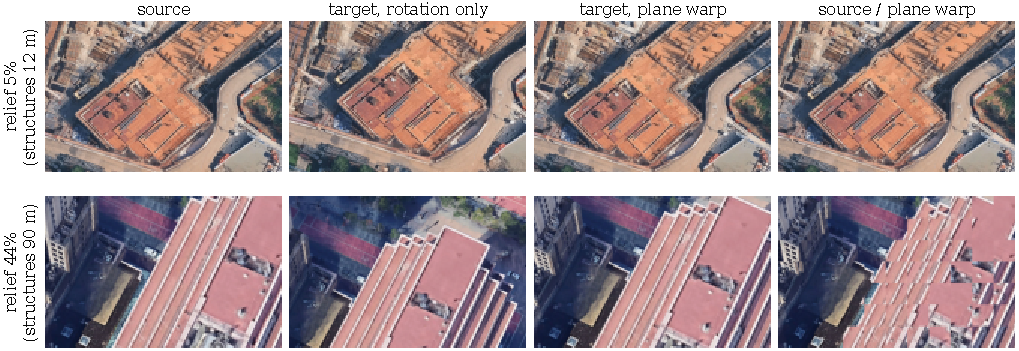
\includegraphics[width=\textwidth]{figures/fig_imagination.pdf}
\caption{\textbf{What the plane-induced warp aligns.} Two test pairs with a baseline of about \fgLowDist\,m and an altitude change of \fgLowDz\,m, warped with the coarse pose (no ground truth). Top: \fgLowRelief\% relief; the rotation alone leaves the change of scale and position, the plane-induced warp aligns the views to \fgLowRes\,px (median over the matches). Bottom: one of the tallest scenes of the test set (\fgHighRelief\% relief, a \fgHighStruct\,m tower); the street is aligned, the roof is displaced by parallax (\fgHighRes\,px), and the tile-wise matcher still returns \fgHighInl{} inliers, which the epipolar re-estimation uses. Last column: checkerboard of the source and the plane-warped target.}
\label{fig:imagination}
\end{figure*}

\begin{table}[t]
\centering
\caption{\textbf{Accuracy against scene relief} (6{,}193 test pairs). Relief: height of the tallest matched structures over the flight height. $S$: that height in metres (median). Res.: median displacement between the imagined and the real view. I / II: coarse / refined stage, camera frame.}
\label{tab:planarity}
\footnotesize
\setlength{\tabcolsep}{2.6pt}
\begin{tabular}{@{}lrrrcccccc@{}}
\toprule
& & $S$ & Res. & \multicolumn{2}{c}{\SRd@1\,m} & \multicolumn{2}{c}{\SRe@1\,m} & \multicolumn{2}{c}{$\dpsi$ MAE} \\
Relief & Pairs & (m) & (px) & I & II & I & II & I & II \\
\midrule
$<$2\% & 34 & 4 & 27.1 & 29.4 & 52.9 & 11.8 & 26.5 & 1.74 & 1.18 \\
2-5\% & 447 & 9 & 12.4 & 51.0 & 71.1 & 28.0 & 58.4 & 0.93 & 0.45 \\
5-10\% & 3683 & 17 & 7.1 & 75.2 & 86.3 & 61.9 & 82.7 & 0.37 & 0.12 \\
10-15\% & 1426 & 25 & 7.3 & 79.0 & 85.1 & 69.3 & 82.5 & 0.25 & 0.09 \\
15-20\% & 330 & 38 & 7.8 & 77.3 & 83.9 & 67.0 & 80.0 & 0.27 & 0.12 \\
20-30\% & 191 & 51 & 8.6 & 78.5 & 87.4 & 70.2 & 84.8 & 0.29 & 0.07 \\
$\geq$30\% & 82 & 79 & 11.6 & 73.2 & 79.3 & 63.4 & 74.4 & 0.22 & 0.15 \\
\bottomrule
\end{tabular}
\end{table}

\begin{table}[t]
\centering
\caption{\textbf{Accuracy against the larger tilt of the pair} (top), \textbf{the height of the source camera above the ground} (middle) \textbf{and the baseline-to-height ratio} (bottom). Same pairs and columns as \cref{tab:planarity}.}
\label{tab:planarity_tilt}
\footnotesize
\setlength{\tabcolsep}{4pt}
\begin{tabular}{@{}lrrcccc@{}}
\toprule
& & Res. & \multicolumn{2}{c}{\SRd@1\,m} & \multicolumn{2}{c}{\SRe@1\,m} \\
Bin & Pairs & (px) & I & II & I & II \\
\midrule
0-15$^\circ$ & 798 & 5.7 & 92.2 & 93.4 & 89.2 & 92.5 \\
15-25$^\circ$ & 1397 & 6.3 & 83.2 & 88.7 & 75.0 & 86.5 \\
25-35$^\circ$ & 1924 & 7.6 & 76.5 & 84.6 & 62.0 & 80.9 \\
35-45$^\circ$ & 2074 & 10.0 & 59.2 & 78.4 & 41.0 & 71.2 \\
\midrule
190-210\,m & 1231 & 7.8 & 75.1 & 81.7 & 62.4 & 77.7 \\
210-230\,m & 3114 & 7.3 & 74.1 & 86.9 & 61.8 & 82.7 \\
230-250\,m & 1773 & 7.1 & 75.6 & 84.9 & 61.8 & 80.5 \\
$\geq$250\,m & 62 & 8.6 & 43.5 & 37.1 & 22.6 & 30.6 \\
\midrule
$<$3\% & 113 & 14.0 & 67.3 & 80.5 & 36.3 & 63.7 \\
3-6\% & 1016 & 7.6 & 71.8 & 86.6 & 56.6 & 80.7 \\
6-9\% & 1898 & 7.8 & 70.5 & 82.1 & 57.6 & 77.9 \\
9-12\% & 1799 & 7.0 & 75.7 & 83.9 & 63.5 & 80.5 \\
$\geq$12\% & 1367 & 7.2 & 80.0 & 87.7 & 69.6 & 84.9 \\
\bottomrule
\end{tabular}
\end{table}


\noindent\textbf{Accuracy against relief.} \Cref{tab:planarity} bins the test pairs by relief. The refinement improves every bin. Its gain in endpoint success is largest on the flattest scenes, +\plGainA{} points \ci{\plGainALo}{\plGainAHi} below 5\% relief, and remains +\plGainC{} \ci{\plGainCLo}{\plGainCHi} between 10\% and 20\% and +\plGainD{} \ci{\plGainDLo}{\plGainDHi} above 20\%. Between 5\% and 30\% of relief, the refined success is flat (\SRd{} between \plMidSRdLo\% and \plMidSRdHi\%), and the displacement between the imagined and the real view stays at about \plResMid\,px. This displacement is mostly the parallax of the matched structures, not the error of the coarse pose: when the warp is computed from the true pose instead (\rgOracleN{} pairs, \cref{tab:raw_geometry}), its median only falls from \rgOursSubRes\,px to \rgOracleRes\,px. It does not follow the relief $S/g$ (Spearman \plSpearRes), because it reflects the typical height of the matched points above the ground rather than the tallest structure. Two regimes are harder. (i) The \plFlatN{} pairs below 5\% of relief are the hardest for \emph{both} stages (coarse \SRd{} \plFlatSiSRd\%, refined \plFlatSiiSRd\%): a nearly planar scene is the ill-conditioned case of two-view geometry discussed in Sec.~4.2, the coarse pose is less accurate there (residual of \plFlatRes\,px), and this is precisely where the plane-induced warp is most faithful and brings its largest gain. (ii) Above 30\% of relief (\plTallN{} pairs) the refined \SRd{} is \plTallSiiSRd\%, a few points below the middle bins. We therefore find no evidence that relief, within the range present in PairUAV, is what limits the refinement.

\noindent\textbf{Tilt, flight height and baseline.} \Cref{tab:planarity_tilt} shows stronger effects than relief. The accuracy decreases with the tilt of the more oblique camera: from \plTiltLoSiiSRd\% to \plTiltHiSiiSRd\% in \SRd{} after refinement, the coarse stage dropping from \plTiltLoSiSRd\% to \plTiltHiSiSRd\%; oblique pairs are the ones on which the refinement helps most. And the \plHighN{} pairs whose source camera is more than 250\,m above the ground are poorly handled by both stages (\plHighSiSRd\% and \plHighSiiSRd\%): the flight-height cue and the bounds on $h$ (\cref{sec:cands,sec:imag}) are calibrated on the training distribution, and DreamNav should not be expected to work at a flight height that differs markedly from it without the height being provided, as it is for the real photographs of \cref{sec:real}. Finally, the shortest baselines, below 3\% of the flight height (\plShortN{} pairs), are the hardest for the coarse stage in endpoint terms (\plShortSiSRe\%) and gain the most from the refinement (\plShortSiiSRe\%).

\noindent\textbf{Scope.} PairUAV views are taken from about 200 to 240\,m above the ground with tilts up to $45^\circ$. The windows and balconies of the introduction motivate why metre-level accuracy is needed at the end of an approach; they do not describe the viewing geometry of the benchmark, and Fig.~1 should not be read as a claim about close-range flight along a facade. In that regime a vertical surface dominates the view, the ground may not be visible, and a ground-plane warp would not align the two images. The closed form of Eq.~(5) would still apply to the facade plane, with a different $\mathbf{n}$ and $h$, but we have not evaluated it and make no claim about it. The real photographs of Sec.~5.3, taken 60\,m above a village, have about 3.7 times the relative relief of PairUAV for the same structures; the refinement still improves on them (\cref{sec:real}).
